\documentclass[preprint, 3p,
authoryear]{elsarticle} %review=doublespace preprint=single 5p=2 column
%%% Begin My package additions %%%%%%%%%%%%%%%%%%%

\usepackage[hyphens]{url}

  \journal{To be confirmed} % Sets Journal name

\usepackage{graphicx}
%%%%%%%%%%%%%%%% end my additions to header

\usepackage[T1]{fontenc}
\usepackage{lmodern}
\usepackage{amssymb,amsmath}
% TODO: Currently lineno needs to be loaded after amsmath because of conflict
% https://github.com/latex-lineno/lineno/issues/5
\usepackage{lineno} % add
\usepackage{ifxetex,ifluatex}
\usepackage{fixltx2e} % provides \textsubscript
% use upquote if available, for straight quotes in verbatim environments
\IfFileExists{upquote.sty}{\usepackage{upquote}}{}
\ifnum 0\ifxetex 1\fi\ifluatex 1\fi=0 % if pdftex
  \usepackage[utf8]{inputenc}
\else % if luatex or xelatex
  \usepackage{fontspec}
  \ifxetex
    \usepackage{xltxtra,xunicode}
  \fi
  \defaultfontfeatures{Mapping=tex-text,Scale=MatchLowercase}
  \newcommand{\euro}{€}
\fi
% use microtype if available
\IfFileExists{microtype.sty}{\usepackage{microtype}}{}
\usepackage[]{natbib}
\bibliographystyle{plainnat}

\usepackage{graphicx}
\ifxetex
  \usepackage[setpagesize=false, % page size defined by xetex
              unicode=false, % unicode breaks when used with xetex
              xetex]{hyperref}
\else
  \usepackage[unicode=true]{hyperref}
\fi
\hypersetup{breaklinks=true,
            bookmarks=true,
            pdfauthor={},
            pdftitle={Social needs for transport and gaps in transit service: new GTFS tools; Appendix materials},
            colorlinks=false,
            urlcolor=blue,
            linkcolor=magenta,
            pdfborder={0 0 0}}

\setcounter{secnumdepth}{5}
% Pandoc toggle for numbering sections (defaults to be off)


% tightlist command for lists without linebreak
\providecommand{\tightlist}{%
  \setlength{\itemsep}{0pt}\setlength{\parskip}{0pt}}




\usepackage{subfig}
\usepackage{booktabs}
\usepackage{longtable}
\usepackage{array}
\usepackage{multirow}
\usepackage{wrapfig}
\usepackage{float}
\usepackage{colortbl}
\usepackage{pdflscape}
\usepackage{tabu}
\usepackage{threeparttable}
\usepackage{threeparttablex}
\usepackage[normalem]{ulem}
\usepackage{makecell}
\usepackage{xcolor}



\begin{document}


\begin{frontmatter}

  \title{Social needs for transport and gaps in transit service: new
GTFS tools; Appendix materials}
    \author[Public Transport Research Group (PTRG)]{James Reynolds%
  %
  \fnref{1}}
   \ead{james.reynolds@monash.edu} 
    \author[Public Transport Research Group (PTRG)]{Graham Currie%
  \corref{cor1}%
  \fnref{2}}
   \ead{graham.currie@monash.edu} 
    \author[Public Transport Research Group (PTRG)]{Yanda Qu%
  %
  \fnref{3}}
   \ead{yanda.qu@monash.edu} 
      \affiliation[Public Transport Research Group (PTRG)]{
    organization={Public Transport Research Group (PTRG), Institute of
Transport Studies, Department of Civil Engineering Engineering, Monash
University},addressline={Clayton
Campus},city={Melbourne},postcode={3800},state={Victoria},country={Australia},}
    \cortext[cor1]{Corresponding author}
    \fntext[1]{Research Fellow}
    \fntext[2]{Professor}
    \fntext[3]{PhD Student}
  
  \begin{abstract}
  Methods of identifying spatial areas where gaps between transit supply
  (accounting for both frequency and coverage) and social needs for
  transport needs are large have previously been presented in research
  literature (Currie 2010). However, this approach does not appear to
  have been widely adopted in practice or received much further
  attention from researchers. This may be due to the challenges
  associated with assessing transit supply levels prior to the
  widespread availability of electronic schedule data, but GTFS datasets
  are now provided by many operators. This paper reports the development
  of an R package of tools for using GTFS datasets for needs-gap
  analysis. Results for Melbourne in 2016 and 2021 are also presented,
  and show similar patterns as in the 2006 results reported in Currie
  (2010), with lower supply levels in outer areas and away from the rail
  network. The number of residents living in areas with Very High needs
  but Very Low or Zero transit supply has increased by 140\% from
  139,004 (4.2\%) in 2006 to 333,887 people (6.8\%) in 2021, while
  Melbourne's overall population increased by only 46\% (3.4m to 4.9m).
  The paper also briefly revists a case study of an early-2010s
  development in the outer south-east suburbs, reported in Delbosc et al
  (2015), finding that there have been positive changes in service level
  at this local scale, but that needs-gaps and lack of services appear
  to remain a challenge. While Melbourne may be an outlier in terms of
  population growth and (low) density, these results might suggest that
  providing even a basic level of transit-based movility to those in
  need may have only become more difficult. Directions for further
  research and limitations are also identified.
  \end{abstract}
    \begin{keyword}
    social needs \sep public transport \sep social transit \sep spatial
analysis \sep 
    GTFS
  \end{keyword}
  
 \end{frontmatter}

\begin{figure}

{\centering \subfloat[Week starting the date of the 2016 census\label{fig:Greater_Melbourne_CCD_2016_appendix-1}]{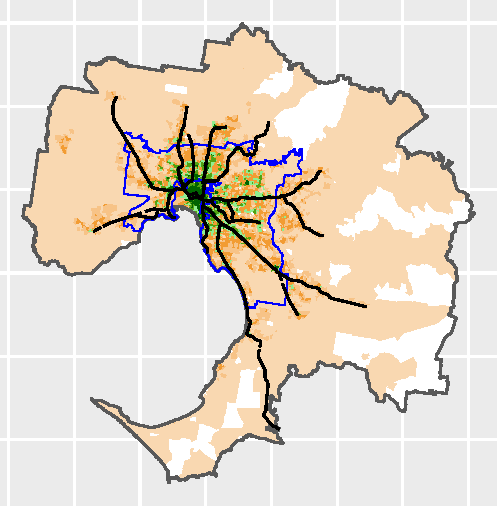
\includegraphics{ReynoldsCurrieQu2024_appendix_files/figure-latex/Greater_Melbourne_CCD_2016_appendix-1} }\subfloat[Week starting the date of the 2021 census\label{fig:Greater_Melbourne_CCD_2016_appendix-2}]{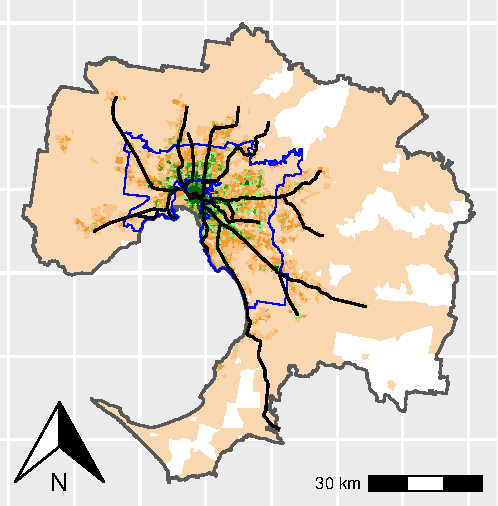
\includegraphics{ReynoldsCurrieQu2024_appendix_files/figure-latex/Greater_Melbourne_CCD_2016_appendix-2} }

}

\caption{Melbourne: Transport Supply Categories by CCD for 2006 extents, overlayed with suburban railway lines (black) and inner, middle and outer suburban boundary (blue)}\label{fig:Greater_Melbourne_CCD_2016_appendix}
\end{figure}

\begin{table}

\caption{\label{tab:Greater_Melbourne_SA1_2016_by_SA4}Greater Melbourne 2016: SA1s in each Transport Supply category by SA4}
\centering
\fontsize{8}{10}\selectfont
\begin{tabular}[t]{>{\raggedright\arraybackslash}p{1.75cm}|>{\raggedleft\arraybackslash}p{1cm}|>{\raggedleft\arraybackslash}p{1cm}|>{\raggedleft\arraybackslash}p{1cm}|>{\raggedleft\arraybackslash}p{1cm}|>{\raggedleft\arraybackslash}p{1cm}|>{\raggedleft\arraybackslash}p{1cm}|>{\raggedleft\arraybackslash}p{1cm}|>{\raggedright\arraybackslash}p{1cm}|>{\raggedleft\arraybackslash}p{1cm}|>{\raggedleft\arraybackslash}p{1.25cm}}
\hline
Transport Supply & Inner & Inner East & Inner South & North East & North West & Outer East & South East & West & M'ton Pen. & Total\\
\hline
Zero Supply & 0.0\%     (0) & 0.0\%   (1) & 0.0\%   (5) & 0.5\%    (48) & 0.4\%  (43) & 0.4\%    (42) & 1.0\%   (101) & 0.2\%    (23) & 0.6\%  (63) & 3.2\%    (326)\\
\hline
Very Low & 0.1\%    (10) & 0.5\%  (50) & 0.7\%  (70) & 2.5\%   (257) & 2.1\% (215) & 5.0\%   (511) & 4.6\%   (473) & 3.7\%   (377) & 3.9\% (399) & 23.0\%  (2,362)\\
\hline
Low & 0.4\%    (44) & 0.9\%  (95) & 1.4\% (142) & 2.8\%   (288) & 2.4\% (243) & 3.2\%   (329) & 5.0\%   (518) & 5.3\%   (541) & 1.6\% (162) & 23.0\%  (2,362)\\
\hline
Below average & 1.0\%   (105) & 2.4\% (249) & 2.9\% (298) & 3.1\%   (319) & 2.2\% (231) & 2.8\%   (284) & 4.0\%   (411) & 3.9\%   (399) & 0.6\%  (66) & 23.0\%  (2,362)\\
\hline
Above average & 1.1\%   (111) & 1.8\% (186) & 1.8\% (184) & 1.0\%   (103) & 0.7\%  (70) & 0.6\%    (60) & 1.1\%   (114) & 1.2\%   (122) & 0.1\%   (9) & 9.3\%    (959)\\
\hline
High & 2.7\%   (279) & 1.7\% (175) & 1.6\% (168) & 1.0\%   (107) & 0.3\%  (31) & 0.4\%    (39) & 0.7\%    (70) & 0.8\%    (86) & 0.0\%   (4) & 9.3\%    (959)\\
\hline
Very High & 6.7\%   (685) & 0.8\%  (86) & 0.7\%  (75) & 0.4\%    (41) & 0.1\%   (7) & 0.0\%     (1) & 0.2\%    (16) & 0.5\%    (48) & 0.0\%   (0) & 9.3\%    (959)\\
\hline
Total & 12.0\% (1,234) & 8.2\% (842) & 9.2\% (942) & 11.3\% (1,163) & 8.2\% (840) & 12.3\% (1,266) & 16.6\% (1,703) & 15.5\% (1,596) & 6.8\% (703) & 100.0\% (10,289)\\
\hline
\end{tabular}
\end{table}

\begin{figure}
\centering
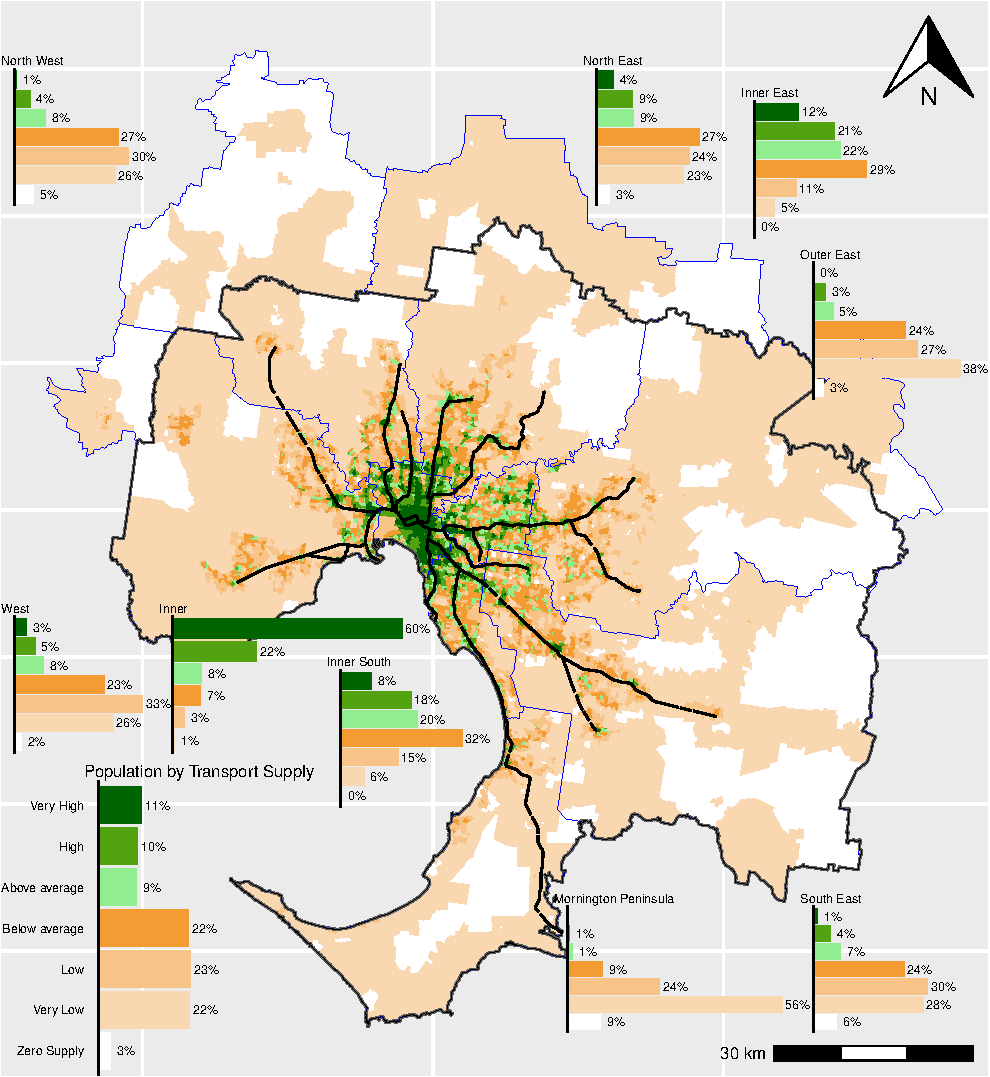
\includegraphics{ReynoldsCurrieQu2024_appendix_files/figure-latex/Greater_Melbourne_SA12016_plot_appendix-1.pdf}
\caption{Greater Melbourne 2016: Transport Supply by SA1, overlayed with
suburban rail network (black), SA4 boundaries (blue) and 2006 Melbourne
extents (black)}
\end{figure}

\begin{table}

\caption{\label{tab:Greater_Melbourne_SA1_2021_by_SA4}Greater Melbourne 2016: SA1s in each Transport Supply category by SA4}
\centering
\fontsize{8}{10}\selectfont
\begin{tabular}[t]{>{\raggedright\arraybackslash}p{1.75cm}|>{\raggedleft\arraybackslash}p{1cm}|>{\raggedleft\arraybackslash}p{1cm}|>{\raggedleft\arraybackslash}p{1cm}|>{\raggedleft\arraybackslash}p{1cm}|>{\raggedleft\arraybackslash}p{1cm}|>{\raggedleft\arraybackslash}p{1cm}|>{\raggedleft\arraybackslash}p{1cm}|>{\raggedright\arraybackslash}p{1cm}|>{\raggedleft\arraybackslash}p{1cm}|>{\raggedleft\arraybackslash}p{1.25cm}}
\hline
Transport Supply & Inner & Inner East & Inner South & North East & North West & Outer East & South East & West & M'ton Pen. & Total\\
\hline
Zero Supply & 0.0\%     (0) & 0.0\%   (1) & 0.0\%   (5) & 0.6\%    (71) & 0.5\%  (55) & 0.4\%    (44) & 1.2\%   (142) & 1.0\%   (112) & 0.5\%  (59) & 4.3\%    (489)\\
\hline
Very Low & 0.1\%    (13) & 0.5\%  (54) & 0.5\%  (63) & 2.7\%   (307) & 2.2\% (254) & 4.6\%   (523) & 5.0\%   (576) & 4.4\%   (504) & 3.5\% (398) & 23.4\%  (2,692)\\
\hline
Low & 0.4\%    (48) & 0.9\% (108) & 1.3\% (147) & 2.8\%   (322) & 2.4\% (279) & 3.2\%   (368) & 5.3\%   (608) & 5.7\%   (653) & 1.4\% (158) & 23.4\%  (2,691)\\
\hline
Below average & 1.1\%   (130) & 2.7\% (310) & 2.9\% (333) & 3.2\%   (363) & 2.6\% (297) & 2.3\%   (261) & 4.1\%   (470) & 3.8\%   (437) & 0.8\%  (90) & 23.4\%  (2,691)\\
\hline
Above average & 1.2\%   (137) & 1.4\% (160) & 1.8\% (210) & 0.9\%   (101) & 0.5\%  (63) & 0.4\%    (49) & 1.0\%   (114) & 1.1\%   (128) & 0.1\%  (13) & 8.5\%    (975)\\
\hline
High & 3.0\%   (345) & 1.5\% (172) & 1.4\% (161) & 0.8\%    (95) & 0.2\%  (22) & 0.3\%    (29) & 0.5\%    (55) & 0.8\%    (93) & 0.0\%   (2) & 8.5\%    (974)\\
\hline
Very High & 6.6\%   (763) & 0.6\%  (65) & 0.5\%  (57) & 0.2\%    (26) & 0.0\%   (5) & 0.0\%     (0) & 0.2\%    (19) & 0.3\%    (40) & 0.0\%   (0) & 8.5\%    (975)\\
\hline
Total & 12.5\% (1,436) & 7.6\% (870) & 8.5\% (976) & 11.2\% (1,285) & 8.5\% (975) & 11.1\% (1,274) & 17.3\% (1,984) & 17.1\% (1,967) & 6.3\% (720) & 100.0\% (11,487)\\
\hline
\end{tabular}
\end{table}

\begin{table}

\caption{\label{tab:Greater_Melbourne_2016_2021_ratio_SA1_table}Greater Melbourne: Share of 2021 SA1s by change in transit service (2016 vs 2021) by SA4 region}
\centering
\fontsize{8}{10}\selectfont
\begin{tabular}[t]{>{\raggedright\arraybackslash}p{1.75cm}|>{\raggedleft\arraybackslash}p{1cm}|>{\raggedleft\arraybackslash}p{1cm}|>{\raggedleft\arraybackslash}p{1cm}|>{\raggedleft\arraybackslash}p{1cm}|>{\raggedleft\arraybackslash}p{1cm}|>{\raggedleft\arraybackslash}p{1cm}|>{\raggedleft\arraybackslash}p{1cm}|>{\raggedright\arraybackslash}p{1cm}|>{\raggedleft\arraybackslash}p{1cm}|>{\raggedleft\arraybackslash}p{1.25cm}}
\hline
Change & Inner & Inner East & Inner South & North East & North West & Outer East & South East & West & M'ton Pen. & Total\\
\hline
New service & 0.0\%     (0) & 0.0\%   (0) & 0.0\%   (0) & 0.2\%    (20) & 0.7\%  (79) & 0.0\%     (1) & 1.0\%   (113) & 0.8\%    (87) & 0.1\%   (6) & 2.7\%    (306)\\
\hline
Increased 30\% or more & 0.0\%     (5) & 0.0\%   (1) & 0.7\%  (83) & 0.9\%   (107) & 1.5\% (173) & 0.1\%    (10) & 2.6\%   (293) & 2.5\%   (290) & 1.3\% (154) & 9.7\%  (1,116)\\
\hline
Increased 10 to 30\% & 0.9\%   (104) & 0.1\%   (7) & 0.9\%  (99) & 0.8\%    (95) & 1.2\% (133) & 0.5\%    (54) & 1.5\%   (173) & 2.0\%   (231) & 0.4\%  (49) & 8.2\%    (945)\\
\hline
Increased 5 to 10\% & 1.4\%   (166) & 0.2\%  (28) & 1.0\% (120) & 0.8\%    (90) & 0.7\%  (75) & 0.6\%    (69) & 1.0\%   (120) & 2.0\%   (233) & 0.2\%  (23) & 8.0\%    (924)\\
\hline
Increased 3 to 5\% & 1.6\%   (185) & 0.5\%  (58) & 0.6\%  (71) & 1.3\%   (147) & 1.1\% (122) & 0.5\%    (63) & 0.9\%   (104) & 1.8\%   (210) & 0.3\%  (32) & 8.6\%    (992)\\
\hline
Increased 1 to 3\% & 2.4\%   (281) & 1.3\% (152) & 1.2\% (142) & 1.9\%   (214) & 0.9\% (107) & 0.9\%   (101) & 1.5\%   (176) & 2.4\%   (271) & 0.7\%  (76) & 13.2\%  (1,520)\\
\hline
Within 1\% & 2.5\%   (286) & 3.9\% (444) & 1.9\% (223) & 2.6\%   (295) & 1.2\% (138) & 5.8\%   (661) & 5.4\%   (620) & 3.0\%   (347) & 2.3\% (261) & 28.5\%  (3,275)\\
\hline
Reduced 1 to 3\% & 1.0\%   (114) & 0.8\%  (94) & 0.5\%  (63) & 0.8\%    (89) & 0.3\%  (32) & 0.8\%    (92) & 0.7\%    (77) & 0.4\%    (44) & 0.4\%  (42) & 5.6\%    (647)\\
\hline
Reduced 3 to 10\% & 1.8\%   (212) & 0.5\%  (61) & 0.9\% (100) & 0.9\%   (105) & 0.2\%  (28) & 0.9\%   (102) & 0.5\%    (58) & 0.7\%    (79) & 0.1\%  (15) & 6.6\%    (760)\\
\hline
Reduced 10\% or more & 0.7\%    (83) & 0.2\%  (24) & 0.6\%  (70) & 0.5\%    (52) & 0.3\%  (33) & 0.7\%    (77) & 0.9\%   (108) & 0.5\%    (63) & 0.0\%   (3) & 4.5\%    (513)\\
\hline
Service withdrawn (magenta) & 0.0\%     (0) & 0.0\%   (0) & 0.0\%   (0) & 0.0\%     (4) & 0.0\%   (1) & 0.0\%     (3) & 0.0\%     (3) & 0.0\%     (4) & 0.0\%   (0) & 0.1\%     (15)\\
\hline
Never served (black) & 0.0\%     (0) & 0.0\%   (1) & 0.0\%   (5) & 0.6\%    (67) & 0.5\%  (54) & 0.4\%    (41) & 1.2\%   (139) & 0.9\%   (108) & 0.5\%  (59) & 4.1\%    (474)\\
\hline
Total & 12.5\% (1,436) & 7.6\% (870) & 8.5\% (976) & 11.2\% (1,285) & 8.5\% (975) & 11.1\% (1,274) & 17.3\% (1,984) & 17.1\% (1,967) & 6.3\% (720) & 100.0\% (11,487)\\
\hline
\end{tabular}
\end{table}

\begin{figure}
\centering
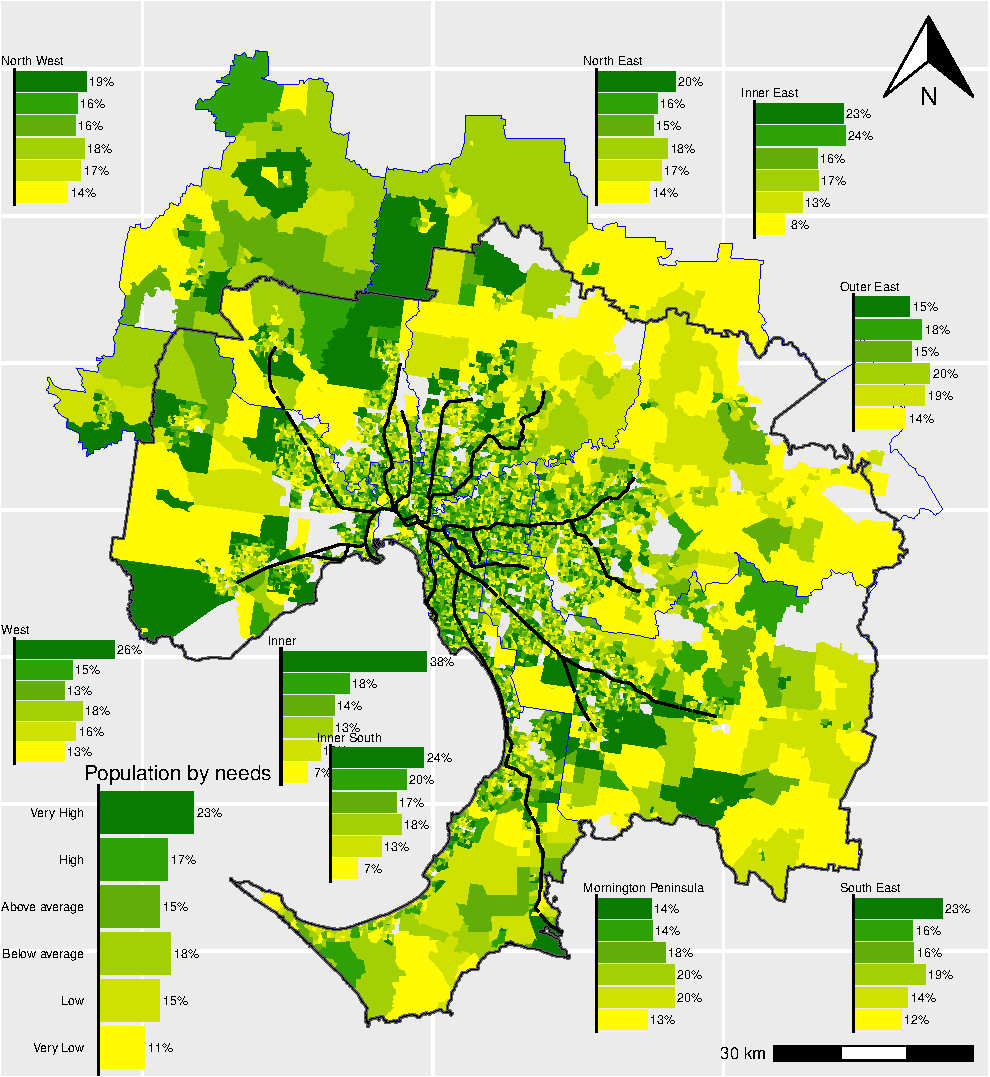
\includegraphics{ReynoldsCurrieQu2024_appendix_files/figure-latex/Greater_Melbourne_2016_social_needs_appendix-1.pdf}
\caption{Distribution of categories of composite social need index
scores in 2016 overlayed with: 2006 Greater Melbourne boundary (black);
SA4 boundaries (blue) and suburban railway lines (black).}
\end{figure}

\begin{table}

\caption{\label{tab:Greater_Melbourne_2016_needs_gap_zones}Greater Melbourne 2016, SA1s within each SI and Combined Needs Index grouping}
\centering
\fontsize{7}{9}\selectfont
\begin{tabular}[t]{l|r|r|r|r|r|r|r}
\hline
transit\_supply & Very Low & Low & Below average & Above average & High & Very High & Total\\
\hline
Zero Supply & 4.8\%    (91) & 3.5\%    (66) & 2.5\%    (47) & 2.4\%    (34) & 2.0\%    (28) & 3.2\%    (46) & 3.1\%   (312)\\
\hline
Very Low & 26.1\%   (497) & 23.2\%   (442) & 20.9\%   (397) & 20.4\%   (290) & 19.8\%   (281) & 22.5\%   (319) & 22.3\% (2,226)\\
\hline
Low & 24.1\%   (458) & 24.5\%   (467) & 24.4\%   (464) & 22.3\%   (317) & 21.7\%   (308) & 19.7\%   (279) & 23.0\% (2,293)\\
\hline
Below average & 24.9\%   (473) & 24.5\%   (467) & 24.1\%   (459) & 23.8\%   (338) & 23.2\%   (329) & 17.6\%   (249) & 23.2\% (2,315)\\
\hline
Above average & 7.4\%   (140) & 9.2\%   (175) & 10.2\%   (194) & 10.5\%   (149) & 10.6\%   (150) & 9.2\%   (131) & 9.4\%   (939)\\
\hline
High & 6.5\%   (123) & 7.5\%   (142) & 10.7\%   (203) & 10.2\%   (145) & 12.0\%   (170) & 10.9\%   (155) & 9.4\%   (938)\\
\hline
Very High & 6.4\%   (121) & 7.6\%   (144) & 7.3\%   (139) & 10.3\%   (146) & 10.7\%   (152) & 16.9\%   (239) & 9.4\%   (941)\\
\hline
Total & 100.0\% (1,903) & 100.0\% (1,903) & 100.0\% (1,903) & 100.0\% (1,419) & 100.0\% (1,418) & 100.0\% (1,418) & 100.0\% (9,964)\\
\hline
\end{tabular}
\end{table}

\begin{table}

\caption{\label{tab:Greater_Melbourne_2021_needs_gap_zones}Greater Melbourne 2021, SA1s within each SI and Combined Needs Index grouping}
\centering
\fontsize{8}{10}\selectfont
\begin{tabular}[t]{>{\raggedright\arraybackslash}p{2.0cm}|>{\raggedleft\arraybackslash}p{1.25cm}|>{\raggedleft\arraybackslash}p{1.25cm}|>{\raggedleft\arraybackslash}p{1.25cm}|>{\raggedleft\arraybackslash}p{1.25cm}|>{\raggedleft\arraybackslash}p{1.25cm}|>{\raggedleft\arraybackslash}p{1.25cm}|>{\raggedleft\arraybackslash}p{1.5cm}}
\hline
\multicolumn{1}{c|}{ } & \multicolumn{6}{c|}{Combined Needs Index Category} & \multicolumn{1}{c}{ } \\
\cline{2-7}
transit\_supply & Very Low & Low & Below average & Above average & High & Very High & Total\\
\hline
Zero Supply & 6.4\%   (130) & 4.7\%    (95) & 3.9\%    (79) & 2.9\%    (49) & 3.0\%    (51) & 3.6\%    (61) & 4.2\%    (465)\\
\hline
Very Low & 25.6\%   (521) & 22.2\%   (452) & 21.8\%   (444) & 21.0\%   (352) & 22.0\%   (369) & 24.3\%   (408) & 22.9\%  (2,546)\\
\hline
Low & 23.5\%   (479) & 25.3\%   (514) & 24.6\%   (500) & 24.0\%   (403) & 22.4\%   (376) & 20.6\%   (346) & 23.5\%  (2,618)\\
\hline
Below average & 23.7\%   (483) & 23.7\%   (482) & 24.0\%   (488) & 25.6\%   (430) & 24.6\%   (412) & 20.8\%   (349) & 23.7\%  (2,644)\\
\hline
Above average & 6.9\%   (140) & 8.1\%   (165) & 9.2\%   (188) & 9.4\%   (157) & 9.1\%   (152) & 9.2\%   (154) & 8.6\%    (956)\\
\hline
High & 5.9\%   (120) & 8.0\%   (162) & 9.5\%   (193) & 9.2\%   (154) & 9.7\%   (162) & 9.8\%   (165) & 8.6\%    (956)\\
\hline
Very High & 8.0\%   (163) & 8.1\%   (165) & 7.0\%   (143) & 7.9\%   (133) & 9.2\%   (155) & 11.6\%   (194) & 8.6\%    (953)\\
\hline
Total & 100.0\% (2,036) & 100.0\% (2,035) & 100.0\% (2,035) & 100.0\% (1,678) & 100.0\% (1,677) & 100.0\% (1,677) & 100.0\% (11,138)\\
\hline
\end{tabular}
\end{table}

\begin{figure}
\centering
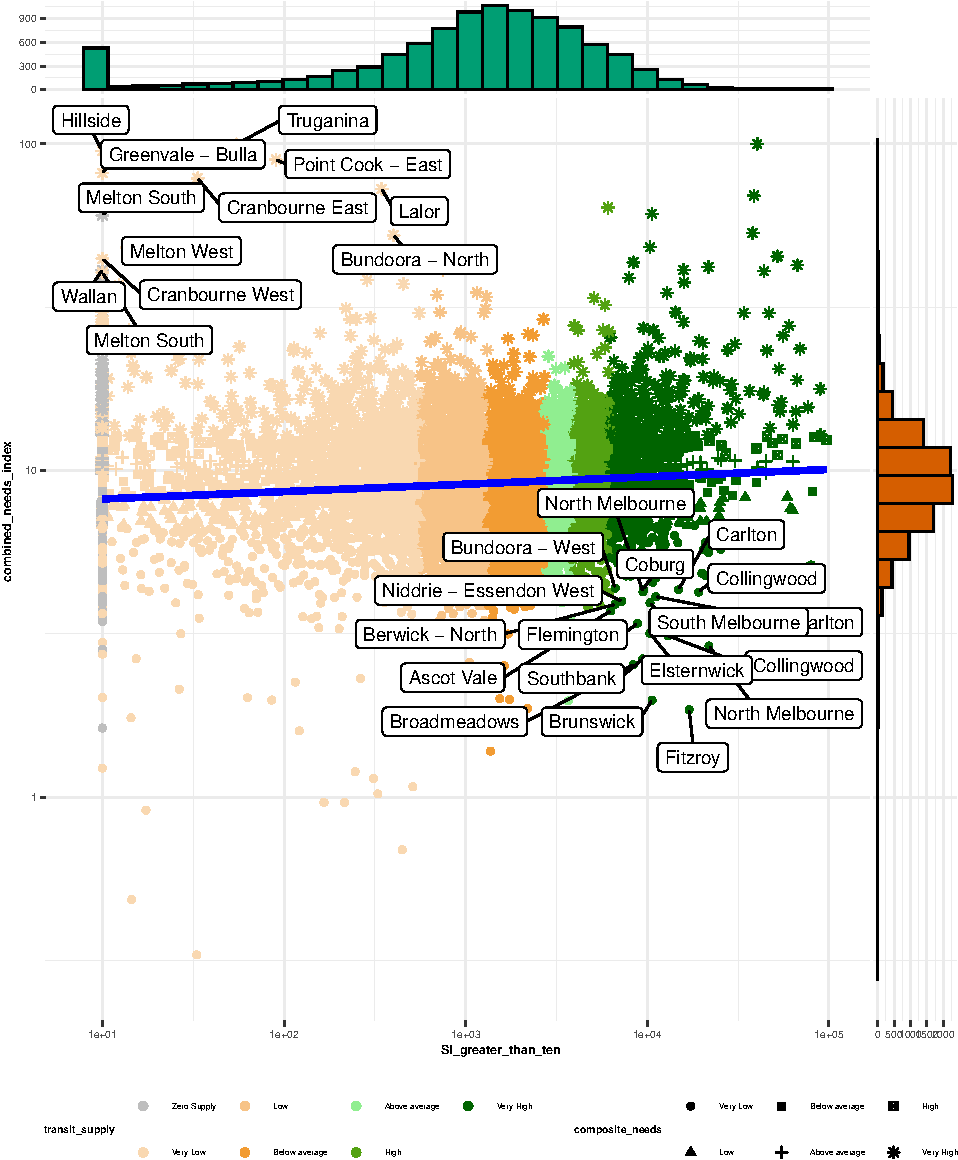
\includegraphics{ReynoldsCurrieQu2024_appendix_files/figure-latex/Greater_Melbourne_2016_needs_gap_scatterplot_figure-1.pdf}
\caption{Greater Melbourne 2016, SI and Combined Needs Index scores,
with SI scores \textless{} 10 rounded up to equal 10.}
\end{figure}

```

\bibliography{References.bib, packages.bib}


\end{document}
